\documentclass[12pt, a4paper]{article}
\usepackage[margin = 1in, top=1.3in]{geometry}
\usepackage[english]{babel}
\usepackage[utf8]{inputenc}
\usepackage{fancyhdr}
\usepackage{amsmath}
\usepackage{bm}
\usepackage{graphicx}
\graphicspath{{./images/}}
\usepackage[font=small,labelfont=bf]{caption}
 
\pagestyle{fancy}
\fancyhf{}
\rhead{\small{Niraj Mahajan (180050069) \\ Raaghav Raaj (180050082)}}
\lhead{CS-215 Assignment-4 : Question 2}
\rfoot{Page 2.\thepage}
 
\begin{document}
\section*{Question 2}
\subsection*{2.1 : Part A}
\hspace{1cm} Given a Mean Vector, and the Covariance Matrix of a Multivariate Gaussian, we need to draw variables from it. \\ 
We have : 
$$\mathbf{X_{2x1} = \boldsymbol{\mu}_{2x1} + A_{2x2}.W_{2x1}}$$
where the covariance matrix = $\mathbf{C = A.A^T}$ \\
Now since the Covariance Matrix is Symmetric and SPD, we have 
$$\mathbf{C = U.S.U^T}$$
\begin{flushright}
where, \textbf{U} = $\begin{bmatrix}
\mathbf{V_1} & \mathbf{V_2} & ... & \mathbf{V_n}
\end{bmatrix} $ and \textbf{S} is diag($\lambda_1,\lambda_2 ... \lambda_n $) \\
where $\mathbf{V_i}$ are eigenvectors and $\lambda_i$ are the corresponding eigenvalues \\
\end{flushright}
Now, consider a symmetric matrix $\mathbf{S_1}$ = $\mathbf{S_1^T}$ = diag($\sqrt{\lambda_1},\sqrt{\lambda_2} ... \sqrt{\lambda_n} $). \\We have
$$\mathbf{C = A.A^T = C = U.S.U^T = U.S_1.S_1^T.U^T = (U.S_1)(U.S_1)^T}$$
Hence, $\mathbf{A = U.S_1}$ \\ \\
Now that we have \textbf{A}, we can easily draw random variables in the following manner: 
\begin{itemize}
\item We can draw 2 Normal Gaussian Random Variables into a 2x1 matrix \textbf{W}.
\item  Since we have our \textbf{A}, which is a 2x2 matrix, we can compute a MVG by the following equation
$$\mathbf{X_{2x1} = \boldsymbol{\mu}_{2x1} + A_{2x2}.W_{2x1}}$$
\end{itemize}

This is the process to draw RV from a MVG with just mean and covariance given!
\newpage
\subsection*{2.2, 2.3 : Part B, Part C}
For every value of N, 100 readings of errors in Mean and Covariance were computed and the respective plots are as follows: \\


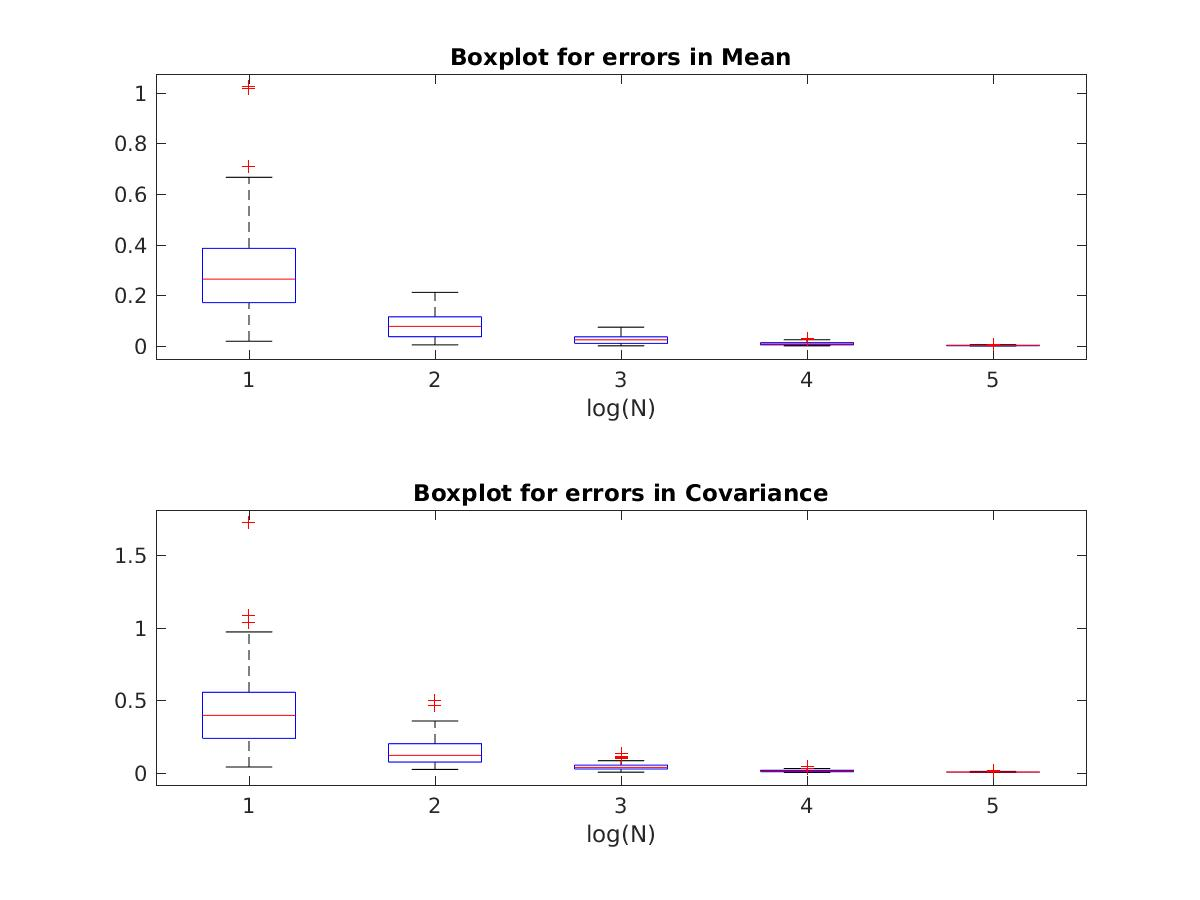
\includegraphics[width=\textwidth, height = 0.6\paperheight]{BoxPlots}


\newpage
\subsection*{2.4 : Part D}
For each N, for every data sample, the scatter plots of the generated data are plotted along with the principal modes of variation of the data. The plots follow: \\

 \noindent The plots of the comparison follow:
 
\noindent 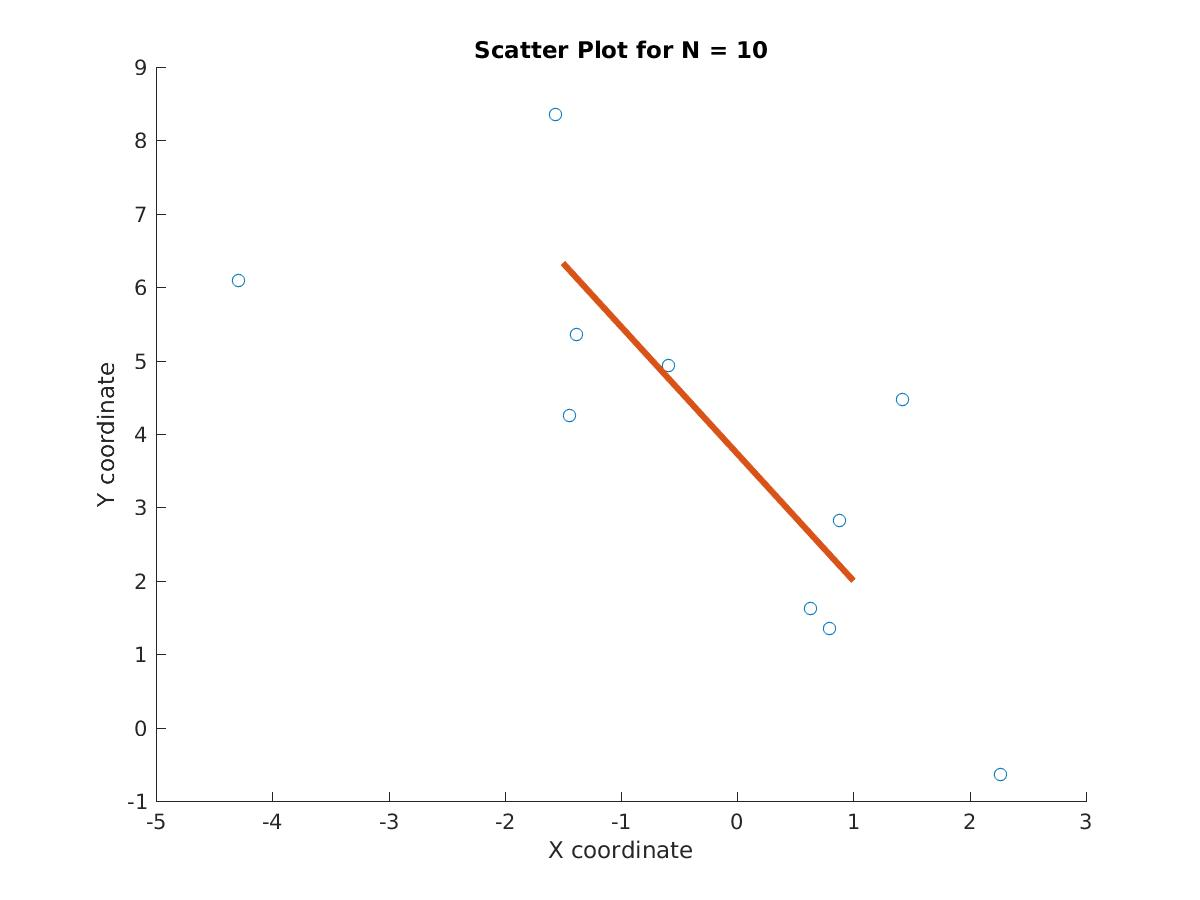
\includegraphics[width=\textwidth, height = 0.25\paperheight]{Scatter_10}
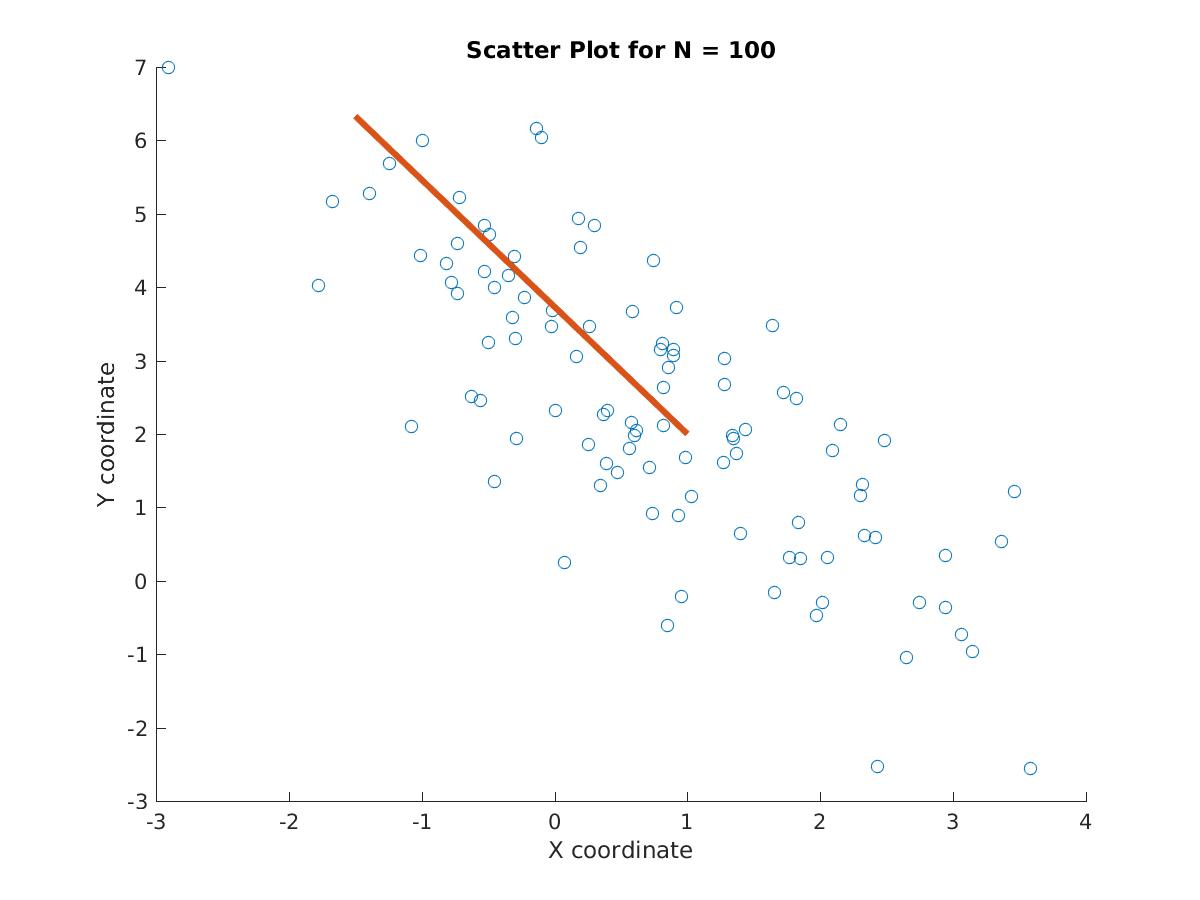
\includegraphics[width=\textwidth, height = 0.25\paperheight]{Scatter_100}
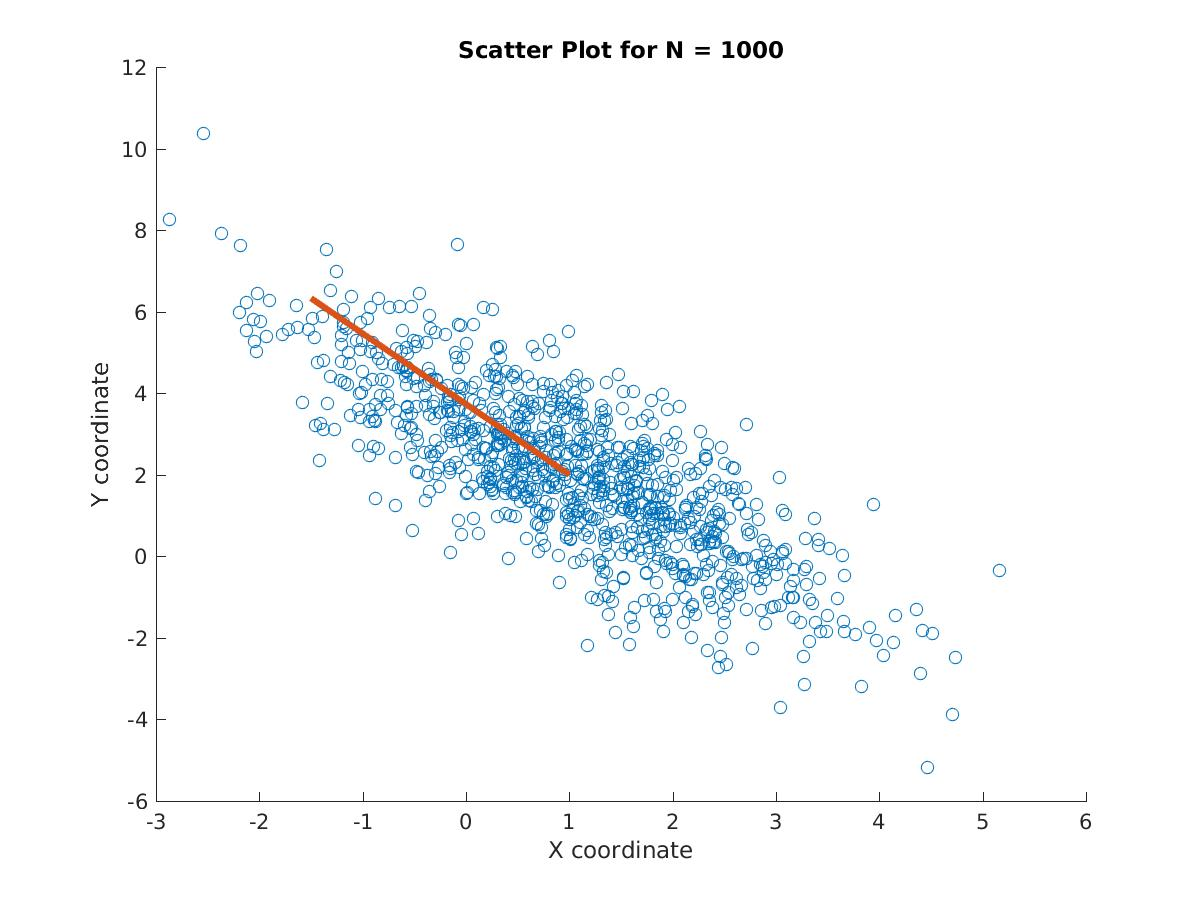
\includegraphics[width=\textwidth, height = 0.25\paperheight]{Scatter_1000}
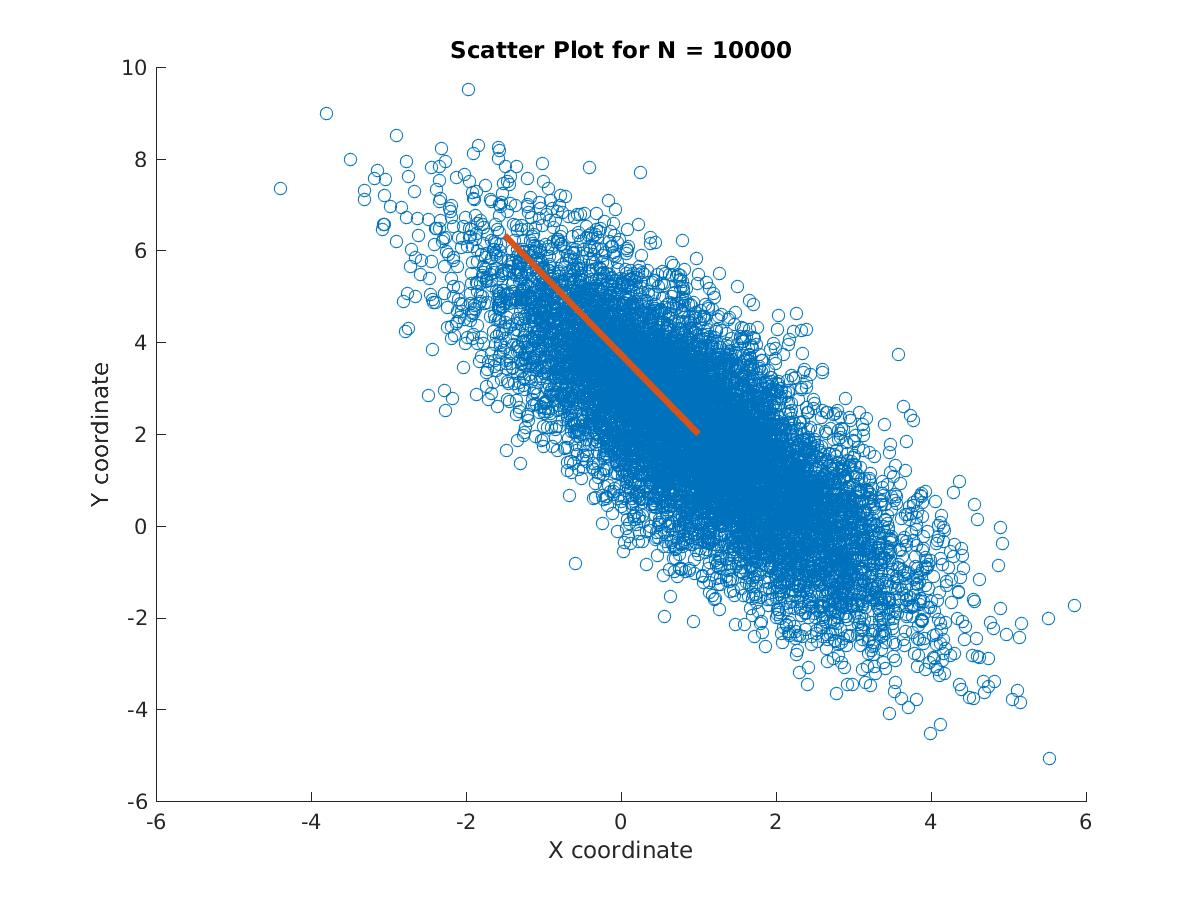
\includegraphics[width=\textwidth, height = 0.25\paperheight]{Scatter_10000}
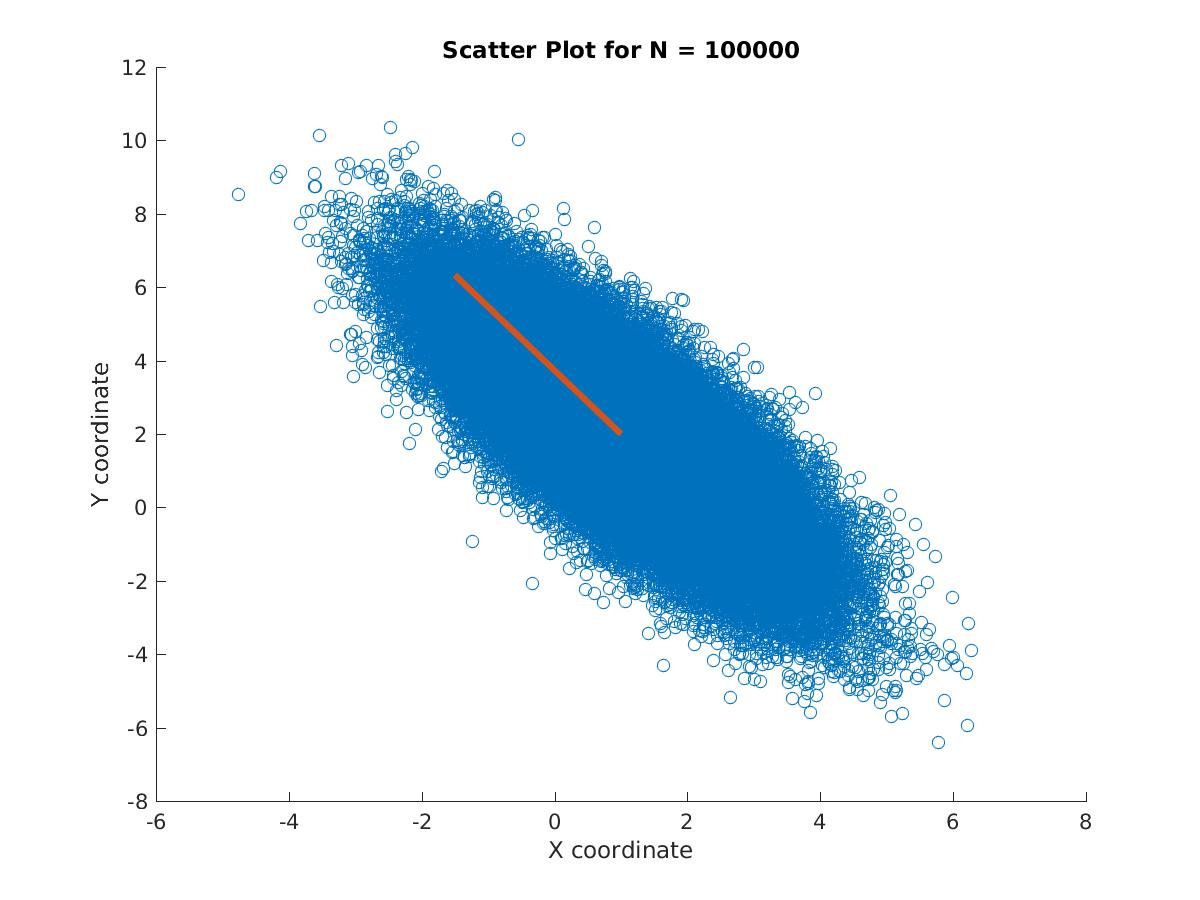
\includegraphics[width=\textwidth, height = 0.25\paperheight]{Scatter_100000}
%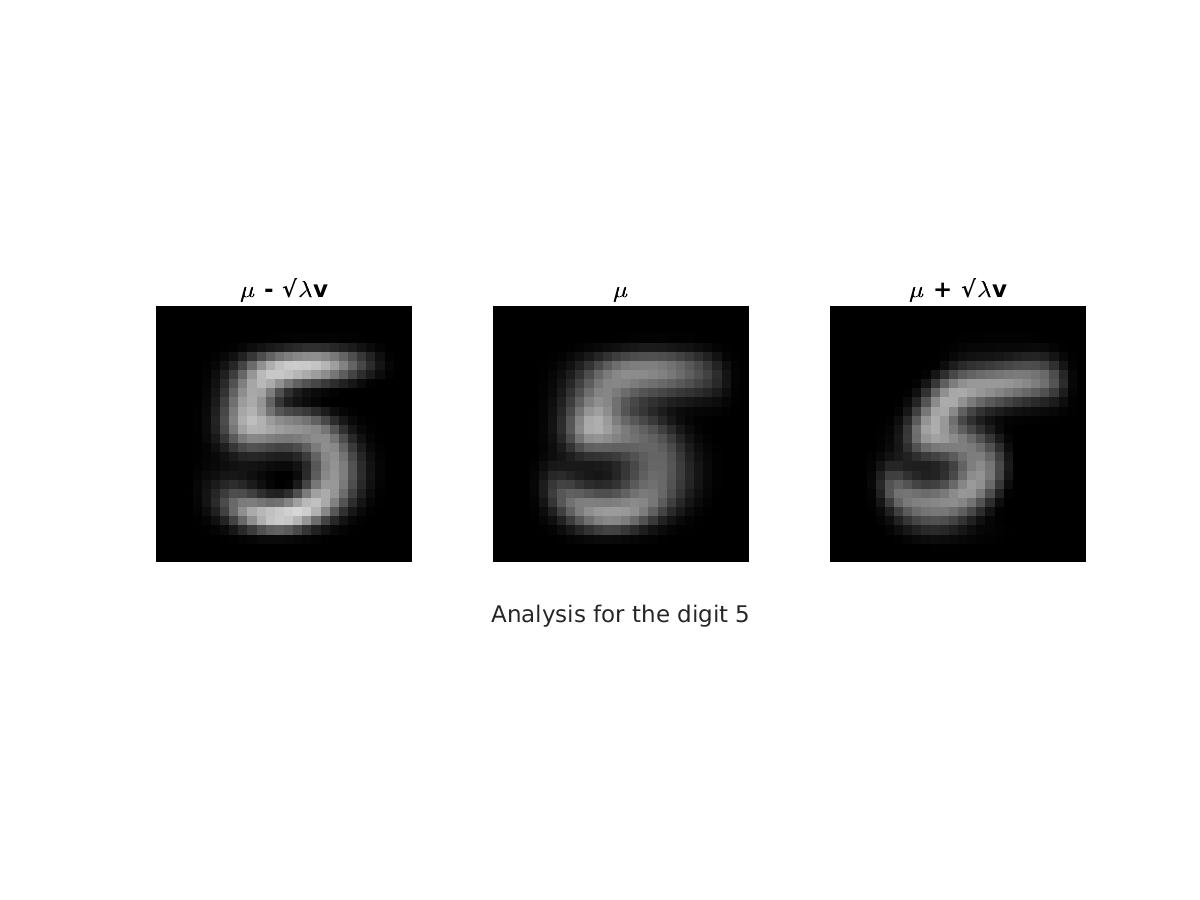
\includegraphics[width=\textwidth, height = 0.25\paperheight]{Comparison_mu_5}
%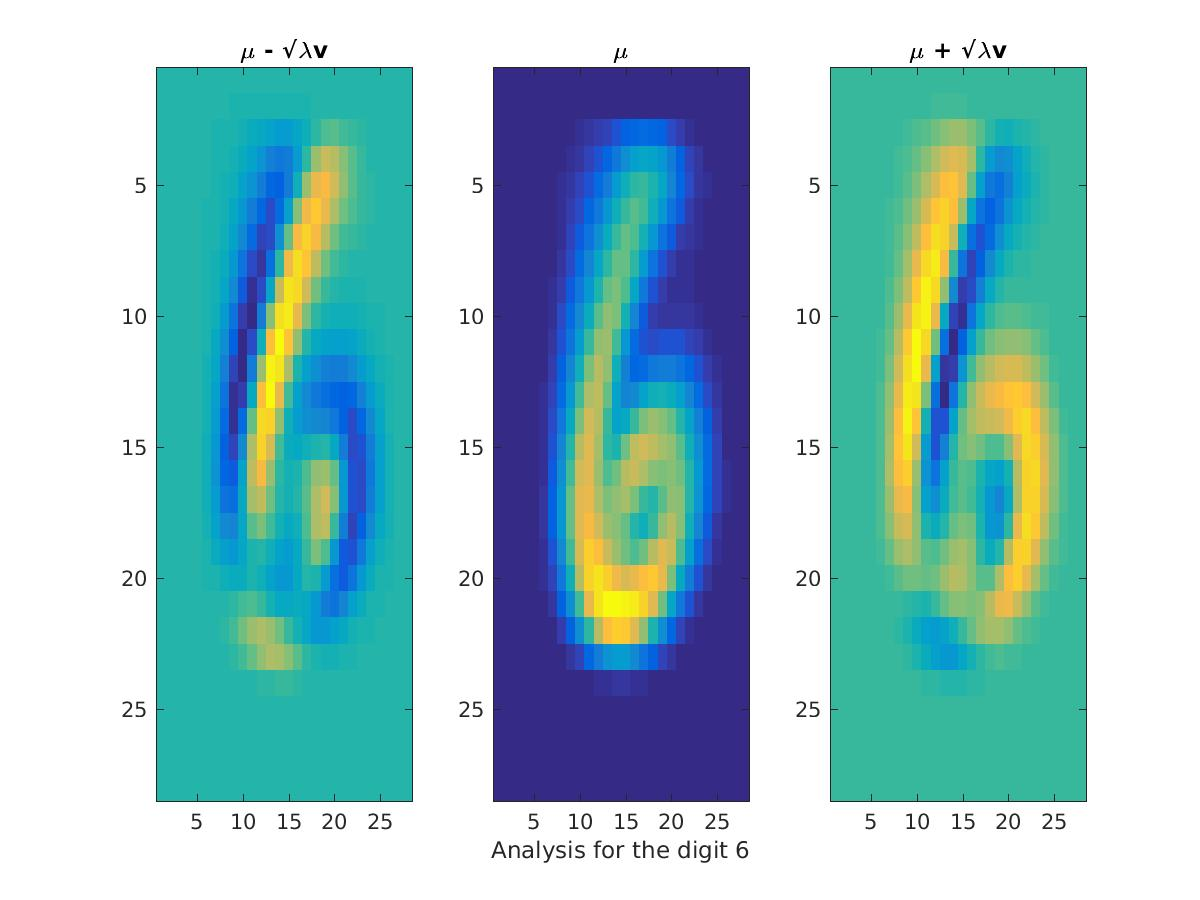
\includegraphics[width=\textwidth, height = 0.25\paperheight]{Comparison_mu_6}
%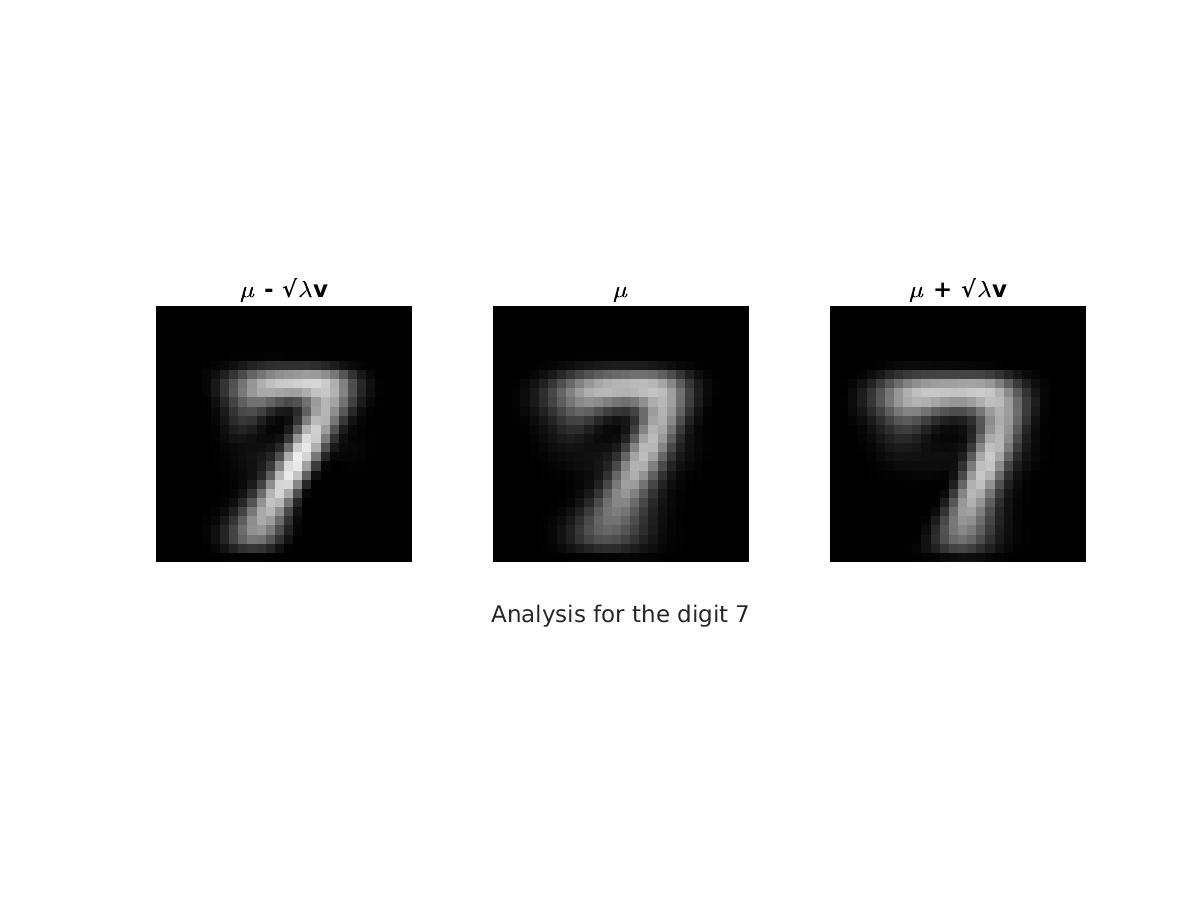
\includegraphics[width=\textwidth, height = 0.25\paperheight]{Comparison_mu_7}
%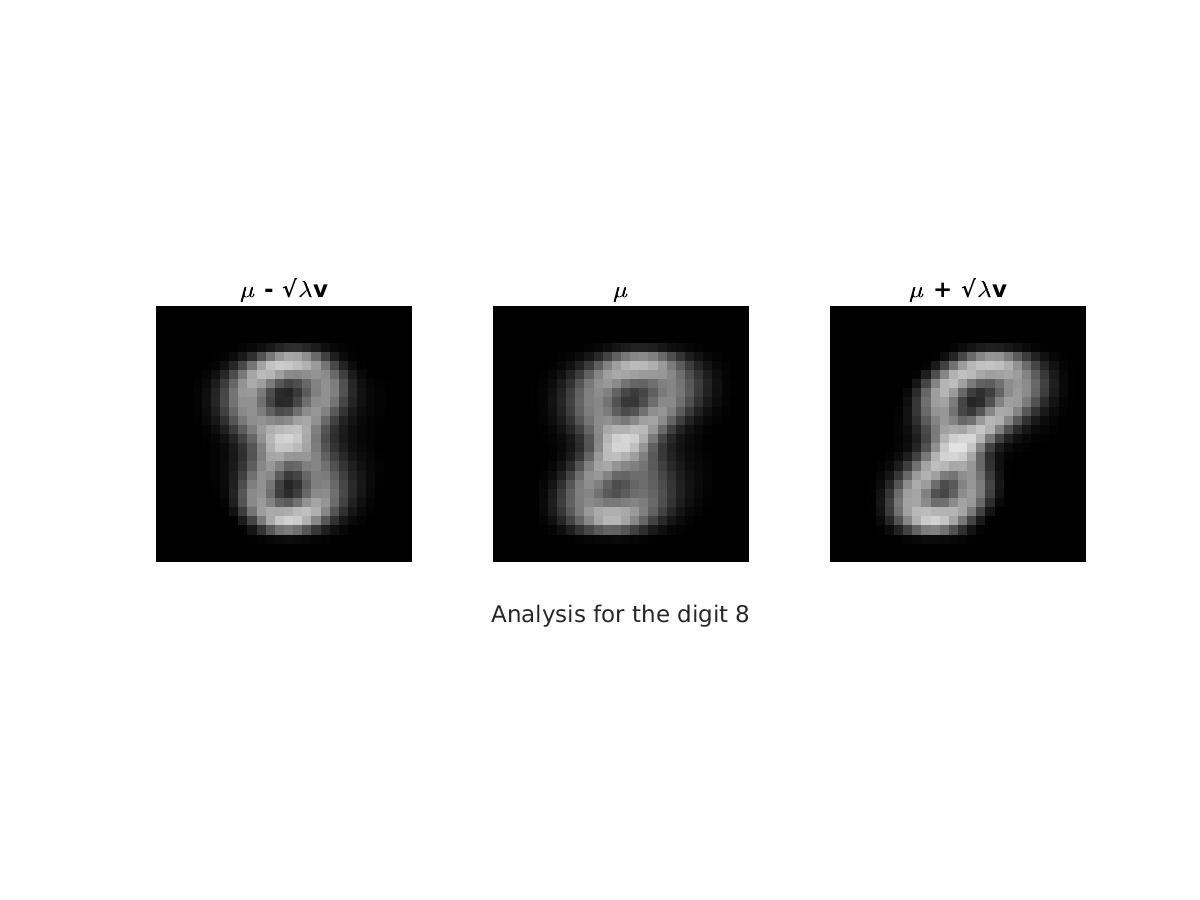
\includegraphics[width=\textwidth, height = 0.25\paperheight]{Comparison_mu_8}
%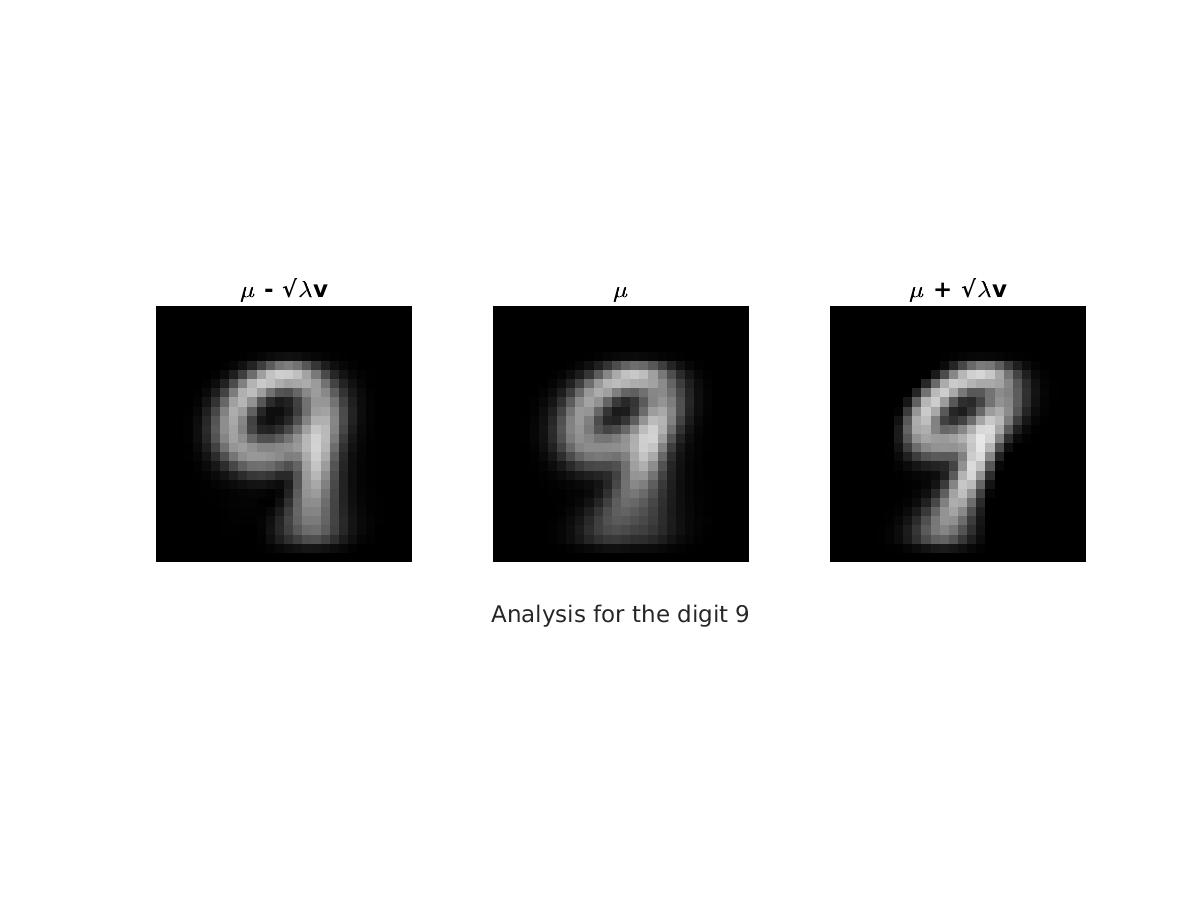
\includegraphics[width=\textwidth, height = 0.25\paperheight]{Comparison_mu_9} 
 
 

\subsection*{2.3 : Usage of Code}
The following are the instructions for the usage of the code:
\begin{itemize}
\item Load the code present in \lq submission/code/q2/q2.m \rq \space.
\item In the same directory are functions implemented like myMean, myCov which return the mean and covariance of appropriate matrices.
\item Simply run the code in \lq q2.m \rq \space and this wil automatically create the required plots.
\item Lines 55, 70 (commented by default) hava a code to save jpg files of the respective plots. Comment/Uncomment these lines appropriately according to need.
\end{itemize}
 
 
\end{document}